%%%%%%%%%%%%%%%%%%%%%%%%%%%%%%%%%%%%%%%%%
% 模板資訊:
% 模板名稱:Ernie's Article
% 版本:1.0 (2023.03.26)
% 作者:莊程翔 Ernie Cheng-Xiang Zhuang
% 編譯器:XeLaTeX -> BibTeX -> XeLaTeX -> XeLaTeX
%
% 製作本模板之目的:
% 由於,LaTeX 對初學者來說不太友善,且 Word 在於數學式及中文排版上不大美觀。因此我製作了這個模板,同時附上清楚明瞭的註解、許多常用且好用的封包,以及客製化設定指令,以便 LaTeX 初學者能夠輕鬆地完成作業、報告甚至是學位論文。
% 如果您有任何問題,可以透過以下兩種方式聯繫我: 
% 1. 網站:https://www.ernie-zhuang.com/contact
% 2. Email:erniezhuang1127@gmail.com
%%%%%%%%%%%%%%%%%%%%%%%%%%%%%%%%%%%%%%%%%

%----------------------------------------------------------------------------------------
%	封包與文檔配置
%----------------------------------------------------------------------------------------

\documentclass[utf8,12pt]{article} % 設定字體大小及 UTF-8 編碼

%%%%%%%%%%%%%%%%%%%%%%%%%%%%%%%%%%%%%%%%%
% 模板資訊:
% 模板名稱:Ernie's Article
% 版本:1.0 (2023.03.26)
% 作者:莊程翔 Ernie Cheng-Xiang Zhuang
% 編譯器:XeLaTeX -> BibTeX -> XeLaTeX -> XeLaTeX
%
% 製作本模板之目的:
% 由於,LaTeX 對初學者來說不太友善,且 Word 在於數學式及中文排版上不大美觀。因此我製作了這個模板,同時附上清楚明瞭的註解、許多常用且好用的封包,以及客製化設定指令,以便 LaTeX 初學者能夠輕鬆地完成作業、報告甚至是學位論文。
% 如果您有任何問題,可以透過以下兩種方式聯繫我: 
% 1. 網站:https://www.ernie-zhuang.com/contact
% 2. Email:erniezhuang1127@gmail.com
%%%%%%%%%%%%%%%%%%%%%%%%%%%%%%%%%%%%%%%%%

%----------------------------------------------------------------------------------------
%	封包與文檔配置
%----------------------------------------------------------------------------------------

% 輸出的字體是以 Type 1 編碼
\usepackage[T1]{fontenc} 

% 自訂字體的封包
\usepackage{fontspec} 

%% 設定英文字體
\setmainfont{Times New Roman} 

%% 設定中文字體
\usepackage{xeCJK}
\setCJKmainfont[AutoFakeBold=3.5 , AutoFakeSlant=0.2, Path = fonts/]{源雲明體.ttf}
\setCJKmonofont[AutoFakeBold=3.5 , AutoFakeSlant=0.2, Path = fonts/]{源雲明體.ttf}
\XeTeXlinebreaklocale "zh"
\XeTeXlinebreakskip = 0pt plus 1pt

% 設定為 A4 紙的大小及上下左右的邊界
\usepackage[left=3.18cm, right=3.18cm, top=2.54cm, bottom=2.54cm]{geometry} 

% 行距,搭配後面得\begin{spacing}{1.5} 及 \end{spacing}
\usepackage{setspace} 

% 每段首行文字空行的封包
\usepackage{indentfirst} 

% 設定空 2 個字元 (2em)
\setlength{\parindent}{2em} 

% 呼叫任意大小字體的封包 (如 13.5pt)
\usepackage{type1cm} 

% 設置節的編號形式 (若不想變更節的樣式,將此以下至 \usepackage{color} 前都以 % 註釋掉。)
\usepackage{titletoc} % 調整節標題的形式
\usepackage[small]{titlesec} % 修改章節字型與大小。(可於中括號中加入 small, sf)
%\usepackage{zhnumber} % 編號為一、二⋯
%\renewcommand\thesection{\zhnum{section}、} % 調整節的編號 (還可以用 \Alph, \alph, Roman, roman)
%\renewcommand\thesubsection{\arabic{subsection}.} % 調整子節的編號
%\renewcommand\thesubsubsection{(\arabic{subsubsection})} % 調整小節的編號
%\makeatletter

% 設置章節編號與章節標題的距離
%\renewcommand\@seccntformat[1]{
%   {\csname the#1\endcsname}\hspace{0em}
%}

% 自訂字體顏色的封包
\usepackage{color} 

%% 自訂顏色
\definecolor{NTHU_Purple}{RGB}{126,35,138}
\definecolor{Default_Blue}{RGB}{52,51,171}

% 數學工具及符號
\usepackage{mathtools, amsmath, amsfonts, amsthm, latexsym} 

% 分別將數學符號間的間隔加大及加粗
\usepackage{newtxtext,newtxmath}

\theoremstyle{definition} % 數學定理及定義的風格,plain, remark, definition, thmsty
\newtheorem{Assum}{\textbf{假設}}
\newtheorem{Axiom}{\textbf{公理}}
\newtheorem{Def}{\textbf{定義}}
\newtheorem{Thm}{\textbf{定理}}
\newtheorem{Lemma}{\textbf{引理}}
\newtheorem{Corol}{\textbf{推論}}
\newtheorem{Property}{\textbf{性質}}
\newtheorem{Proposition}{\textbf{命題}}
\newtheorem{Claim}{\textbf{宣稱}}
\newtheorem{Remark}{\textbf{備註}}
\newtheorem{Note}{\textbf{註記}}
\renewcommand{\proofname}{\rm\textbf{證明}}
%\renewcommand{\qedsymbol}{}

% 打勾 \Checkmark、打叉 \XSolid
\usepackage{bbding} 

% 圖表自動編號的封包
\usepackage[justification=centering]{caption} 
\usepackage[justification=centering, format=hang]{subcaption}

%% 設定圖表編號及標籤的字體大小及字形
\captionsetup[figure]{font=normalsize, labelfont=md}
\captionsetup[table]{font=normalsize, labelfont=md}

% 導入圖形與表格的封包
\usepackage{graphicx}  % \scalebox{} 可用於將過大的表格縮小
\usepackage{booktabs}

% 允許表格的一格能多列呈現的封包
\usepackage{multirow} 

% 可指定表格排版的封包
\usepackage{array}

% 逆時針翻轉表格 90 度
\usepackage{lscape} 

% 長表格
\usepackage{longtable} 

% 表格內數字,以小數點或逗點對齊
\usepackage{dcolumn} 

% 調整圖的位置
\renewcommand{\textfraction}{0.15}
\renewcommand{\topfraction}{0.85}
\renewcommand{\bottomfraction}{0.85}
\renewcommand{\floatpagefraction}{0.60}

% 調整表中數字的對齊方式
\newcolumntype{d}[1]{D{,}{,}{#1}} % 以逗點對齊,應在排表格時鍵入 d{?}
\newcolumntype{.}[1]{D{.}{.}{#1}} % 以小數點對齊,應在排表格時鍵入 .{?}

% 文繞圖
\usepackage{wrapfig} 

% 增加註腳的間隔
\setlength{\footnotesep}{1em} 

% 超連結的封包
\usepackage{url}
\usepackage[colorlinks, bookmarks = false]{hyperref}

%% 設定各種超連結的顏色
\hypersetup{
	linkcolor = black,
	citecolor = blue,
	filecolor = blue,
	urlcolor = blue
} 

% 序列標號
\usepackage{enumerate} 

% 註釋掉大部分的封包
\usepackage{comment}

% 導入 pdf 檔的封包 
\usepackage{pdfpages} % \includepdf[pages=-]{檔名}

% 摘要的封包
\usepackage{abstract} 
\renewcommand{\abstractnamefont}{\Large} % 摘要,兩字的大小

% 附錄的封包
\usepackage{appendix} 

% 引注參考文獻的封包
\usepackage[sort]{natbib}

% 設定手動引注參考文獻的格式
\newcommand\laref{\bigskip\noindent\hangindent=1em} 

% 修改頁眉與頁足
%\usepackage{fancyhdr} 
%\pagestyle{fancy} % 設定頁眉與頁足的顯示風格,有 empty、plain、headings、myheadings、fancy。
%\renewcommand{\sectionmark}[1]{\markright{\thesection#1}} 
%\fancyhead[LO, LE]{}
%\fancyhead[RO, RE]{\rightmark}
%\addtolength{\headheight}{6pt}
%\renewcommand{\footrulewidth}{0pt}
%\extrarowheight=2pt

% 設定中文的標籤
\renewcommand{\figurename}{圖} 
\renewcommand{\tablename}{表} 
\renewcommand{\abstractname}{\textbf{摘要}} 
\renewcommand{\contentsname}{\textbf{目錄}}
\renewcommand{\listfigurename}{\textbf{圖目錄}}
\renewcommand{\listtablename}{\textbf{表目錄}}
\renewcommand{\refname}{\textbf{參考文獻}}
\renewcommand{\appendixpagename}{\Large \textbf{附錄}}
 % 載入封包與文檔配置

%----------------------------------------------------------------------------------------
%	文章資訊
%----------------------------------------------------------------------------------------

% 名稱
\title{\LaTeX{}  Article 如何做?}

% 作者
\author{莊程翔\thanks{國立清華大學經濟學系} \and Ernie Cheng-Xiang Zhuang\thanks{National Tsing Hua University}}

% 日期可以任意輸入大括號內
\date{\today}

\begin{document}

\pagenumbering{roman} % 頁數以小寫羅馬字呈現

%----------------------------------------------------------------------------------------
%	文章標題
%----------------------------------------------------------------------------------------
%
\maketitle 
%
%----------------------------------------------------------------------------------------
%	摘要
%----------------------------------------------------------------------------------------
%
\begin{abstract}\fontsize{12}{20pt}
\begin{spacing}{1.5}
台灣地區歷經經濟發展及教育環境變遷,
高中生在選組上仍明顯存在性別差異,
且隨時間演進並無重大改變。
本研究利用「台灣教育長期追蹤資料庫」(Taiwan Education Panel Survey) 分析性別、學生數學能力及家庭背景對於選組的影響,
我們的實證結果顯示高中生選組偏好存在相當大的歧異,
其中數學成就差距是重要的解釋因素,
但數學對男女的影響並不一致,
而其它家庭背景變數則相對並不重要。
此外雖然女性明顯較男性不傾向選擇自然組,
但性別間稟賦差 距可解釋的部分只佔 16\%–21\%,
性別間選組差異仍大部分無法由男女間稟賦不同所解釋。
最後本研究結果間接反駁女生較不傾向選擇自然組,
乃因其數學能力較差所致之觀點。

\bigskip
\noindent
\textbf{關鍵詞}:高中生選組,數學背景,家庭背景,性別差異

\bigskip
\noindent
\textbf{JEL 分類代號}: I21, I28, J16, J24

\bigskip
\noindent
本摘要取自\href{https://econ.ntu.edu.tw/ter/new/data/new/TER394/TER394-4.pdf}{\citet{郭祐誠2011}}。
\end{spacing}
\end{abstract}
%
%----------------------------------------------------------------------------------------
%	目錄
%----------------------------------------------------------------------------------------
%
\newpage
\fontsize{12}{20pt}
\begin{spacing}{1.5}
\tableofcontents
%
% 圖目錄
\newpage
\listoffigures
%
% 表目錄
\newpage
\listoftables
%
\end{spacing}
%
%----------------------------------------------------------------------------------------
%	一般的文字處裡
%----------------------------------------------------------------------------------------
%
\newpage
\pagenumbering{arabic} % 頁數以數字呈現 
\section{一般的文字處裡}
\begin{spacing}{1.5}
%
研究表明,
漢字的序順並不定一能影閱響讀,
比如當你看這句話後,
才發這現裡的字全是都亂的。

% \textcolor{red}{} 是讓字變紅色, \textbf 是讓字變粗體,\textit 則是變斜體。
\textcolor{red}{Econometrics} is a \textbf{statistical} method used to \textit{estimate} the economic relationship,
test economic theories, and evaluate the effects of government or business policies.

% 引用名言
\begin{quote}
	Pure mathematics is, in its way, the poetry of logical ideas.\\
	(純粹數學,就其本質而言,是邏輯思想的詩篇。)\\
	--- Albert Einstein (愛因斯坦)
\end{quote}
%
\end{spacing}
%
%----------------------------------------------------------------------------------------
%	項目編號及數字編號
%----------------------------------------------------------------------------------------
%
\newpage
\section{項目編號及數字編號}
\begin{spacing}{1.5}
%
\begin{itemize} % 封包 itemize 的 item
\item 這是封包 itemize 的 item
		\begin{enumerate}[a] % 封包 enumerate 的 item,[] 中輸入 a。
			\item Beamer 中,中括號內可以不輸入任何東西,也會有實心圓點,在 Article 則不能這樣輸入
			\item 這是封包 enumerate 的 item,中括號內輸入 a
			\begin{itemize} % 封包 itemize 的 item
				\item 這是第二層 itemize 的 item
				\begin{enumerate}[1] % 封包 enumerate 的 item,[] 中輸入 1。
					\item 這是封包 enumerate 的 item,中括號內輸入 1
					\item 這是封包 enumerate 的 item,中括號內輸入 1
				\end{enumerate}
			\end{itemize}
		\end{enumerate}
\end{itemize}
\end{spacing}
%
%----------------------------------------------------------------------------------------
%	數學
%----------------------------------------------------------------------------------------
%
\section{數學}
%
%----------------------------------------------------------------------------------------
%
\subsection{數學定理}
%
%----------------------------------------------------------------------------------------
%
\begin{spacing}{1.5}
%
\begin{Def}
	一個二次可微分的實數函數$f\left(x\right)$稱為一個凸函數(convex function),
	若$f^{\,\prime\prime}\!\left(x\right)\ge0$對所有$x$;
	同理若$f^{\,\prime\prime}\!\left(x\right)\le0$對所有$x$,
	則稱為凹函數(concave function)。
\end{Def}

\begin{Axiom}
	公理可以用 Axiom 的環境指令。
\end{Axiom}

\begin{Assum}
	假設可以用 Assum 的環境指令。
\end{Assum}

\begin{Thm}
	定理可以用 Thm 的環境指令。
\end{Thm}

\begin{Lemma}
	引理可以用 Lemma 的環境指令。
\end{Lemma}

\begin{Corol}
	推論可以用 Corol 的環境指令。
\end{Corol}

\begin{Property}
	性質可以用 Property 的環境指令。
\end{Property}

\begin{Proposition}
	命題可以用 Proposition 的環境指令。
\end{Proposition}

\begin{Claim}
	宣稱可以用 Claim 的環境指令。
\end{Claim}

\begin{Remark}
	備註可以用 Remark 的環境指令。
\end{Remark}

\begin{Note}
	註記可以用 Note 的環境指令。
\end{Note}

\begin{proof}
	證明可以用 proof 的環境指令。
\end{proof}
%
\end{spacing}
%
%----------------------------------------------------------------------------------------
%
\subsection{數學方程式}
%
%----------------------------------------------------------------------------------------
%
% 數學式中,我們會適時加入符號來增減空隙。
	%% \, 增加 1.5pt 
	%% \! 減少 1.5pt
	%% \: 增加 3pt
	%% \; 增加 5pt
\begin{align}\label{reg}
	\ln\left[\frac{Prob.\left(Y=b|X\right)}{Prob.\left(Y=0|X\right)}\right]
		=\beta_0+\sum_{j=1}^k \beta_{i,j}\,X_{i,j,b|Y=0}+\varepsilon_{i,b|Y=0}
\end{align}
%
\begin{align}\label{var}
	\left(n-1\right)\!S^{\,2} & =  \sum_{i=1}^{n}\left(x_{i}-\widebar{X}\right)^{2} 
		 =  \sum_{i=1}^{n}x_i^{\,2}-n\widebar{X}^{\,2} \notag \\
	\Rightarrow \sum_{i=1}^{n} x_i^{\,2} & =  \left(n-1\right)\!S^{\,2}+\underbrace{n \widebar{X}^{\,2}}_{\text{校正項}}
\end{align}
%
%----------------------------------------------------------------------------------------
%	插入單頁圖片
%----------------------------------------------------------------------------------------
%
\section{圖表製作}
%
%----------------------------------------------------------------------------------------
%
\subsection{單頁圖片}
%
%----------------------------------------------------------------------------------------
%
\begin{figure}[htbp]
	\centering % 置中
	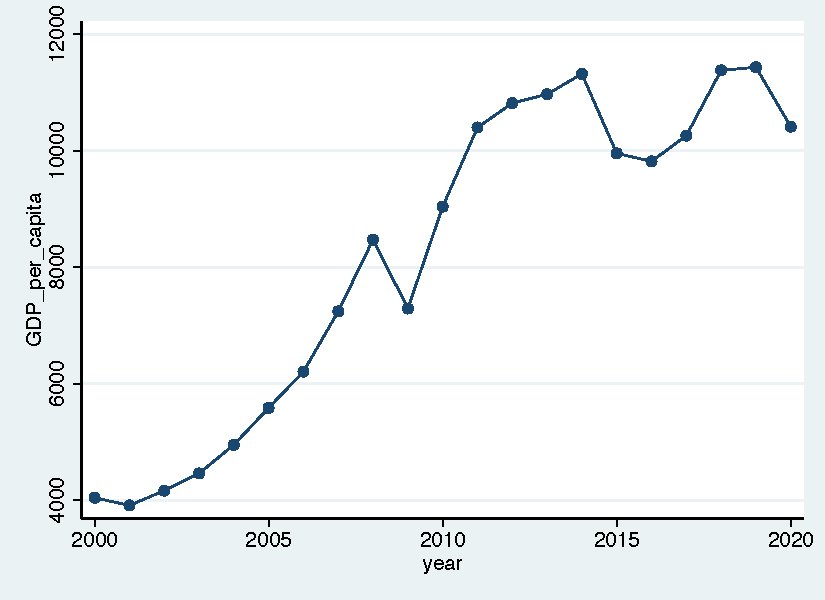
\includegraphics[scale=0.85]{Fig/GDP_per_capita.pdf}\\ % 導入圖片並調整大小
	\hspace{-19em}\footnotesize{資料來源:Worldbank。}\\ % 調整位置並輸入資料來源
	\caption{馬來西亞的GDP per capita (current US\$)} % 圖片名稱
	\label{GDP_per_capita} % 建立圖標籤
\end{figure}
%
%----------------------------------------------------------------------------------------
%
\subsection{群組圖片}
%
%----------------------------------------------------------------------------------------
%
\begin{figure}[htbp]
	\centering 
	\begin{subfigure}[b]{0.45\textwidth} % 調整欄寬
		\centering 
		
\includegraphics[width=\textwidth]{Fig/LaTeX}\\
		\footnotesize{資料來源:
		\href{https://en.wikipedia.org/wiki/LaTeX}{維基百科}。}
		\caption{\LaTeX~1} 
		\label{LaTeX 1} % 建立子圖標籤
	\end{subfigure}
	\hfill
	\begin{subfigure}[b]{0.45\textwidth}
		\centering
		
\includegraphics[width=\textwidth]{Fig/LaTeX}
		\footnotesize{資料來源:
		\href{https://en.wikipedia.org/wiki/LaTeX}{維基百科}。}
		\caption{\LaTeX~2} 
		\label{LaTeX 2} % 建立子圖標籤
	\end{subfigure}
	\par
	\begin{subfigure}[b]{0.45\textwidth} % 調整欄寬
		\centering 
		
\includegraphics[width=\textwidth]{Fig/LaTeX}\\
		\footnotesize{資料來源:
		\href{https://en.wikipedia.org/wiki/LaTeX}{維基百科}。}
		\caption{\LaTeX~3} 
		\label{LaTeX 3} % 建立子圖標籤
	\end{subfigure}
	\hfill
	\begin{subfigure}[b]{0.45\textwidth}
		\centering
		
\includegraphics[width=\textwidth]{Fig/LaTeX}
		\footnotesize{資料來源:
		\href{https://en.wikipedia.org/wiki/LaTeX}{維基百科}。}
		\caption{\LaTeX~4} 
		\label{LaTeX 4} % 建立子圖標籤
	\end{subfigure}	
	\caption{\LaTeX} 
	\label{LaTeX} % 建立圖標籤
\end{figure}
%
%----------------------------------------------------------------------------------------
%
\subsection{文繞圖}
%
%----------------------------------------------------------------------------------------
%
\begin{spacing}{1.5}
%
\begin{wrapfigure}{R}{0.3\textwidth} % 用 R 或 L 控制圖的位置
\centering

\includegraphics[width=0.3\textwidth]{Fig/nthulogo}\\
\footnotesize{資料來源:
		\href{https://www.nthu.edu.tw/files/cis/cis-1.pdf}{國立清華大學}。}
\caption{清華大學 Logo}
\end{wrapfigure}
%
本校成立於民國前一年,校址為北平西郊的清華園,最初名稱為「清華學堂」。

民國三年冬天,梁啟超先生來校演講,引述易經中「天行健君子以自強不息,地勢坤君子以厚德載物」勉勵同學以君子自期,自此以後「自強不息,厚德載物」便成為清華的校訓。

民國十七年,本校校名正式定為國立清華大學。對日抗戰爆發後,遷校昆明,與北京大學、南開大學合組為西南聯合大學,勝利後復員北平。民國四十五年在梅貽琦校長主持下又在台灣新竹建校。

本校畢業校友活躍各界,尤其在學術界,前後共有三位諾貝爾獎得主及一位數學伍爾夫獎得主為清華校友,足見清華光榮的歷史傳統與優良的學風。

清華大學復校初期重點為原子科學,其後則擴展至理工方面,近十幾年來更積極發展人文社會、生命科學、電機資訊與科技管理;漸漸地,清華已成為一文、理、工均衡發展的學府。

民國105年11月1日起,國立清華大學與國立新竹教育大學合併為「國立清華大學」。原「國立新竹教育大學附設實驗國民小學」同時更名為「國立清華大學附設實驗國民小學」。(本文取自:\href{https://www.nthu.edu.tw/about/nthuIntro}{國立清華大學}。)
%
\end{spacing}
%
%----------------------------------------------------------------------------------------
%	加入單頁表格
%----------------------------------------------------------------------------------------
%
%----------------------------------------------------------------------------------------
%
\subsection{單頁表格}
%
%----------------------------------------------------------------------------------------
%
\begin{table}[htbp]
	\centering % 置中
	\caption{公立、私立大學的就學貸款統計差異(108 學年度)} % 表名
	\extrarowheight=2pt % 額外增加每列的寬度
	\label{loan} % 建立表標籤
	\scalebox{1}{ % 將表縮小,不要縮小可以調成 1。
	\begin{tabular}{p{5cm} p{3cm}<{\centering} p{3cm}<{\raggedleft}} % 控制欄寬,及文字對齊方式。
		\toprule
		\midrule
 		& 公立大學 & 私立大學\\
		\midrule
		貸款金額 & 3,121,271,506 & 16,098,465,719 \\
		貸款學生人數 & 55,715 & 187,076 \\
		學生人數 & 439,073 & 774,099 \\
		人均貸款金額 & 56,022 & 86,053 \\
		貸款學生人數/學生人數 & 12.69\% & 24.17\% \\
		\midrule
		\bottomrule
	\end{tabular}
	}
	\par\smallskip
	\hspace{0em}\parbox{0.8\textwidth}{\footnotesize % 調整資料來源及表註的位置、字體大小及文字寬度。
	資料來源:\href{https://helpdreams.moe.edu.tw/hd/upload/20201211_1.pdf}{圓夢助學網}。\par\smallskip
	註:\parbox[t]{0.6\textwidth}{\footnotesize % 記得稍微小於前兩行的 \textwidth
	可在此處增加表格備註。
	}
	}
\end{table}
%
%----------------------------------------------------------------------------------------
%
\subsection{翻轉表格}
%
%----------------------------------------------------------------------------------------
%
\begin{landscape}
\begin{table}[htbp]
\centering
\caption{就讀國立大學與就讀一般大學的羅吉斯迴歸結果}
\label{logit}
\begin{tabular}{lccccccc}
\toprule
\midrule
\multirow{2}{*}{} & \multicolumn{3}{c}{就讀國立大學(相對就讀私立大學)} & \multicolumn{3}{c}{就讀一般大學(相對就讀科技大學)} \\ \cmidrule(r){2-4}  \cmidrule(r){5-7} 
 & (1-1) & (1-2) & (1-3) & (2-1) & (2-2) & (2-3) \\ 
 \midrule
父母的社經地位 &  &  &  &  &  &  \\
\hspace{1em} \multirow{2}{*}{父:低;母:中} & 0.039 & 0.041 & 0.023 & 0.545** & 0.546** & 0.528** \\
 & (0.191) & (0.191) & (0.195) & (0.174) & (0.174) & (0.179) \\
\hspace{1em} \multirow{2}{*}{父:低;母:高} & 0.183 & 0.188 & 0.163 & 0.745*** & 0.748*** & 0.813*** \\
 & (0.200) & (0.200) & (0.205) & (0.190) & (0.190) & (0.197) \\
\hspace{1em} \multirow{2}{*}{父:低;母:無就業} & -0.244+ & -0.239+ & -0.206 & 0.121 & 0.123 & 0.187 \\
 & (0.138) & (0.138) & (0.140) & (0.122) & (0.123) & (0.127) \\
\hspace{1em} \multirow{2}{*}{父:中;母:低} & -0.259 & -0.249 & -0.213 & 0.521 & 0.525 & 0.488 \\
 & (0.443) & (0.444) & (0.446) & (0.385) & (0.386) & (0.396) \\
\hspace{1em} \multirow{2}{*}{父:中、母:中} & 0.356 & 0.356 & 0.387 & 0.864** & 0.865** & 0.846** \\
 & (0.291) & (0.292) & (0.293) & (0.310) & (0.310) & (0.312) \\
\hspace{1em} \multirow{2}{*}{父:中;母:高} & 0.264 & 0.261 & 0.305 & 0.547 & 0.546 & 0.636+ \\
 & (0.385) & (0.385) & (0.388) & (0.378) & (0.378) & (0.387) \\
\hspace{1em} \multirow{2}{*}{父:中;母:無就業} & 0.259 & 0.255 & 0.301 & 0.887* & 0.885* & 0.901* \\
 & (0.332) & (0.333) & (0.335) & (0.374) & (0.374) & (0.376) \\
\hspace{1em} \multirow{2}{*}{父:高;母:低} & 0.346* & 0.338+ & 0.360* & 0.455** & 0.452** & 0.508** \\
 & (0.175) & (0.175) & (0.177) & (0.170) & (0.170) & (0.173) \\
\hspace{1em} \multirow{2}{*}{父:高;母:中} & 0.296+ & 0.295+ & 0.323+ & 1.020*** & 1.021*** & 1.029*** \\
 & (0.178) & (0.178) & (0.179) & (0.180) & (0.180) & (0.182) \\
\hspace{1em} \multirow{2}{*}{父:高;母:高} & 0.447** & 0.445** & 0.473** & 1.466*** & 1.465*** & 1.545*** \\
 & (0.144) & (0.144) & (0.146) & (0.161) & (0.161) & (0.167) \\
 \midrule
\bottomrule
\end{tabular}
\end{table}
\end{landscape}
%
%----------------------------------------------------------------------------------------
%
\subsection{長表格}
%
%----------------------------------------------------------------------------------------
%
\begin{longtable}{@{}crrrr@{}}
\caption{CareerCast 近五年五大最佳職業}\label{CareerCast}\\
%\extrarowheight=2pt 
\toprule
\midrule
排名 & 2021 &  2019 & 2018 & 2017 \\ % 表的首列
\midrule
\endfirsthead % 結束首張表格的表頭設定
%
\multicolumn{5}{l}{承接上頁}\\[2pt] % 除首張表外,皆於左上角呈現承接上頁。
\toprule
\midrule
排名 & 2021 &  2019 & 2018 & 2017 \\ % 除首張表外,也皆呈現表的首列。
\midrule
\endhead % 結束除首張表外的表頭設定。
%
\midrule
\bottomrule
\multicolumn{5}{r}{接續下頁}\\[2pt] % 除了最後一張表外,皆於右下角呈現接續下頁。
\endfoot\\[-10pt]  % 結束除了最後一張表外的表末設定。
\multicolumn{5}{l}{\parbox{0.75\textwidth}{\footnotesize % 此行的寬度會影響到表格的寬度
資料來源:\href{https://helpdreams.moe.edu.tw/hd/upload/20201211_1.pdf}{圓夢助學網}。\par\smallskip
註:\parbox[t]{0.7\textwidth}{\footnotesize % 記得稍微小於前兩行的 \textwidth
1、2020 年 CareerCast 沒有公布年度十大最佳職業。\\
2、粗體為理工科 (STEM) 相關的職業。
}
}
}
\endlastfoot
1 & { 資料科學家} & \textbf{資料科學家}  &  遺傳諮詢師 & \textbf{統計學家} \\
2 & 遺傳諮詢師 & \textbf{統計學家} & \textbf{數學家}  & 醫療服務經理 \\
3 & \textbf{統計學家} & 大學教授  & 大學教授 & \textbf{作業研究分析師}\\
4 & 醫療服務經理 & 職能治療師  & 職能治療師 & \textbf{資訊安全分析師} \\
5 & \textbf{數學家} & 遺傳諮詢師 & \textbf{統計學家} & \textbf{資料科學家} \\
1 & { 資料科學家} & \textbf{資料科學家}  &  遺傳諮詢師 & \textbf{統計學家} \\
2 & 遺傳諮詢師 & \textbf{統計學家} & \textbf{數學家}  & 醫療服務經理 \\
3 & \textbf{統計學家} & 大學教授  & 大學教授 & \textbf{作業研究分析師}\\
4 & 醫療服務經理 & 職能治療師  & 職能治療師 & \textbf{資訊安全分析師} \\
5 & \textbf{數學家} & 遺傳諮詢師 & \textbf{統計學家} & \textbf{資料科學家} \\
1 & { 資料科學家} & \textbf{資料科學家}  &  遺傳諮詢師 & \textbf{統計學家} \\
2 & 遺傳諮詢師 & \textbf{統計學家} & \textbf{數學家}  & 醫療服務經理 \\
3 & \textbf{統計學家} & 大學教授  & 大學教授 & \textbf{作業研究分析師}\\
4 & 醫療服務經理 & 職能治療師  & 職能治療師 & \textbf{資訊安全分析師} \\
5 & \textbf{數學家} & 遺傳諮詢師 & \textbf{統計學家} & \textbf{資料科學家} \\
1 & { 資料科學家} & \textbf{資料科學家}  &  遺傳諮詢師 & \textbf{統計學家} \\
2 & 遺傳諮詢師 & \textbf{統計學家} & \textbf{數學家}  & 醫療服務經理 \\
3 & \textbf{統計學家} & 大學教授  & 大學教授 & \textbf{作業研究分析師}\\
4 & 醫療服務經理 & 職能治療師  & 職能治療師 & \textbf{資訊安全分析師} \\
5 & \textbf{數學家} & 遺傳諮詢師 & \textbf{統計學家} & \textbf{資料科學家} \\
1 & { 資料科學家} & \textbf{資料科學家}  &  遺傳諮詢師 & \textbf{統計學家} \\
2 & 遺傳諮詢師 & \textbf{統計學家} & \textbf{數學家}  & 醫療服務經理 \\
3 & \textbf{統計學家} & 大學教授  & 大學教授 & \textbf{作業研究分析師}\\
4 & 醫療服務經理 & 職能治療師  & 職能治療師 & \textbf{資訊安全分析師} \\
5 & \textbf{數學家} & 遺傳諮詢師 & \textbf{統計學家} & \textbf{資料科學家} \\
1 & { 資料科學家} & \textbf{資料科學家}  &  遺傳諮詢師 & \textbf{統計學家} \\
2 & 遺傳諮詢師 & \textbf{統計學家} & \textbf{數學家}  & 醫療服務經理 \\
3 & \textbf{統計學家} & 大學教授  & 大學教授 & \textbf{作業研究分析師}\\
4 & 醫療服務經理 & 職能治療師  & 職能治療師 & \textbf{資訊安全分析師} \\
5 & \textbf{數學家} & 遺傳諮詢師 & \textbf{統計學家} & \textbf{資料科學家} \\
1 & { 資料科學家} & \textbf{資料科學家}  &  遺傳諮詢師 & \textbf{統計學家} \\
2 & 遺傳諮詢師 & \textbf{統計學家} & \textbf{數學家}  & 醫療服務經理 \\
3 & \textbf{統計學家} & 大學教授  & 大學教授 & \textbf{作業研究分析師}\\
4 & 醫療服務經理 & 職能治療師  & 職能治療師 & \textbf{資訊安全分析師} \\
5 & \textbf{數學家} & 遺傳諮詢師 & \textbf{統計學家} & \textbf{資料科學家} \\
1 & { 資料科學家} & \textbf{資料科學家}  &  遺傳諮詢師 & \textbf{統計學家} \\
2 & 遺傳諮詢師 & \textbf{統計學家} & \textbf{數學家}  & 醫療服務經理 \\
3 & \textbf{統計學家} & 大學教授  & 大學教授 & \textbf{作業研究分析師}\\
4 & 醫療服務經理 & 職能治療師  & 職能治療師 & \textbf{資訊安全分析師} \\
5 & \textbf{數學家} & 遺傳諮詢師 & \textbf{統計學家} & \textbf{資料科學家} \\
1 & { 資料科學家} & \textbf{資料科學家}  &  遺傳諮詢師 & \textbf{統計學家} \\
2 & 遺傳諮詢師 & \textbf{統計學家} & \textbf{數學家}  & 醫療服務經理 \\
3 & \textbf{統計學家} & 大學教授  & 大學教授 & \textbf{作業研究分析師}\\
4 & 醫療服務經理 & 職能治療師  & 職能治療師 & \textbf{資訊安全分析師} \\
5 & \textbf{數學家} & 遺傳諮詢師 & \textbf{統計學家} & \textbf{資料科學家} \\
1 & { 資料科學家} & \textbf{資料科學家}  &  遺傳諮詢師 & \textbf{統計學家} \\
2 & 遺傳諮詢師 & \textbf{統計學家} & \textbf{數學家}  & 醫療服務經理 \\
3 & \textbf{統計學家} & 大學教授  & 大學教授 & \textbf{作業研究分析師}\\
4 & 醫療服務經理 & 職能治療師  & 職能治療師 & \textbf{資訊安全分析師} \\
5 & \textbf{數學家} & 遺傳諮詢師 & \textbf{統計學家} & \textbf{資料科學家} \\
1 & { 資料科學家} & \textbf{資料科學家}  &  遺傳諮詢師 & \textbf{統計學家} \\
2 & 遺傳諮詢師 & \textbf{統計學家} & \textbf{數學家}  & 醫療服務經理 \\
3 & \textbf{統計學家} & 大學教授  & 大學教授 & \textbf{作業研究分析師}\\
4 & 醫療服務經理 & 職能治療師  & 職能治療師 & \textbf{資訊安全分析師} \\
5 & \textbf{數學家} & 遺傳諮詢師 & \textbf{統計學家} & \textbf{資料科學家} \\
1 & { 資料科學家} & \textbf{資料科學家}  &  遺傳諮詢師 & \textbf{統計學家} \\
2 & 遺傳諮詢師 & \textbf{統計學家} & \textbf{數學家}  & 醫療服務經理 \\
3 & \textbf{統計學家} & 大學教授  & 大學教授 & \textbf{作業研究分析師}\\
4 & 醫療服務經理 & 職能治療師  & 職能治療師 & \textbf{資訊安全分析師} \\
5 & \textbf{數學家} & 遺傳諮詢師 & \textbf{統計學家} & \textbf{資料科學家} \\
1 & { 資料科學家} & \textbf{資料科學家}  &  遺傳諮詢師 & \textbf{統計學家} \\
2 & 遺傳諮詢師 & \textbf{統計學家} & \textbf{數學家}  & 醫療服務經理 \\
3 & \textbf{統計學家} & 大學教授  & 大學教授 & \textbf{作業研究分析師}\\
4 & 醫療服務經理 & 職能治療師  & 職能治療師 & \textbf{資訊安全分析師} \\
5 & \textbf{數學家} & 遺傳諮詢師 & \textbf{統計學家} & \textbf{資料科學家} \\
1 & { 資料科學家} & \textbf{資料科學家}  &  遺傳諮詢師 & \textbf{統計學家} \\
2 & 遺傳諮詢師 & \textbf{統計學家} & \textbf{數學家}  & 醫療服務經理 \\
3 & \textbf{統計學家} & 大學教授  & 大學教授 & \textbf{作業研究分析師}\\
4 & 醫療服務經理 & 職能治療師  & 職能治療師 & \textbf{資訊安全分析師} \\
5 & \textbf{數學家} & 遺傳諮詢師 & \textbf{統計學家} & \textbf{資料科學家} \\
1 & { 資料科學家} & \textbf{資料科學家}  &  遺傳諮詢師 & \textbf{統計學家} \\
2 & 遺傳諮詢師 & \textbf{統計學家} & \textbf{數學家}  & 醫療服務經理 \\
3 & \textbf{統計學家} & 大學教授  & 大學教授 & \textbf{作業研究分析師}\\
4 & 醫療服務經理 & 職能治療師  & 職能治療師 & \textbf{資訊安全分析師} \\
5 & \textbf{數學家} & 遺傳諮詢師 & \textbf{統計學家} & \textbf{資料科學家} \\
\midrule
\bottomrule
\end{longtable}
%
%----------------------------------------------------------------------------------------
%	引注
%----------------------------------------------------------------------------------------
%
\section{引注}
%
%----------------------------------------------------------------------------------------
%
\begin{spacing}{1.5}
%
\begin{itemize}
	\item 我們在內文中要提及前面的圖、表或方程式時,應該這樣引注:
	\begin{itemize}
		\item 「圖 $\backslash$ref\{label 內的名字\}」,
			即可出現圖 \ref{GDP_per_capita} 和圖 \ref{LaTeX}。
		\item 「子圖 $\backslash$ref\{label 內的名字\}」,
			即可出現圖 \ref{LaTeX 1}、圖 \ref{LaTeX 2}、圖 \ref{LaTeX 3} 與圖 \ref{LaTeX 4}。
		\item 「表 $\backslash$ref\{label 內的名字\}」,
			即可出現表 \ref{loan} 、表 \ref{logit} 與表 \ref{CareerCast}。
		\item 「式 ($\backslash$ref\{label 內的名字\})」,
				即可出現式 (\ref{reg}) 和式 (\ref{var})。
	\end{itemize}
	\item 另外,引用參考文獻的方法:
	\begin{itemize}
		\item 將文獻作者當作主詞時使用時:\textbackslash citet\{給定的標籤\}。
		\begin{itemize}
			\item 舉例來說:\citet{Ernie1}、\citet{melitz2003} 與 \citet{sin1996}。
		\end{itemize}	
		\item 行文末端作為補充說明時:\textbackslash citep\{給定的標籤\}。
		\begin{itemize}
			\item 舉例來說:\citep{Ernie1}、\citep{melitz2003} 與 \citep{sin1996}。
		\end{itemize}
		\item 注意,使用 bibtex 的好處,它只會幫您輸入使用到的文獻至參考文獻處。(例如,ref.bib 中有一篇 Ernie2 的文章沒有引用)
		\item 但要注意,\textcolor{red}{\LaTeX{} bibtex 的引用格式僅適用於英文},目前我想到一個較有效率的方法是:
		\begin{enumerate}[1]
			\item 分別建立一個含有所有與題目相關的中文加英文的 bib 檔,
			另外也分別根據語言各建立一個檔案。(因此,共有 3 個檔案。)
			\item 先於\textbackslash bibliography\{\} 的大括號中引入雙語的 bib 檔。
			\item 在文章撰寫完畢,準備提交時先將此 tex 檔存檔,並另外複製一份檔案,針對新檔案做修改。 (避免以後修改時,文獻會有所增減。)
			\item 從生成的 pdf 檔中,複製中文文獻的部分,手動加入於 \textbackslash bibliography\{\} 後一行。(針對另存的 tex 檔。)
			\item 加入的方法為,\textbackslash laref 中文文獻。
		\end{enumerate}
		\item 另外,提醒使用 bib 檔,執行編譯器的順序為 XeLaTeX $\rightarrow$ BibTeX $\rightarrow$ XeLaTeX  $\rightarrow$ XeLaTeX (多執行幾次,確保結果都有完整呈現。)
		\item 最後,本文會故意引入雙語的 bib 檔,讓您確認中文也會依照英文格式編排。
	\end{itemize}	
\end{itemize}

引注的好處是內文有所更動時,不用一直手動調整編號。
%
\end{spacing}
%
%----------------------------------------------------------------------------------------
%	參考文獻
%----------------------------------------------------------------------------------------
%
%\newpage
%\fancyhead[RO, RE]{參考文獻}
\addcontentsline{toc}{section}{\textbf{參考文獻}}
\bibliographystyle{apalike}
\bibliography{ref}
%
\laref \textcolor{red}{以下是手動輸入的。}\par
\laref 莊程翔 (2023)。遇到中文文獻只能夠靠手動引述,因為標點符號不支援1。\emph{期刊名稱},31(3):203--255。\par
\laref 郭祐誠與許聖章 (2011)。數學能力與性別對高中學生選組之影響。\emph{經濟論文叢刊},39(4):541–591。
%
%----------------------------------------------------------------------------------------
%	附錄
%----------------------------------------------------------------------------------------
%
%\newpage
%\fancyhead[RO, RE]{附錄}
\addcontentsline{toc}{section}{\textbf{附錄}}
\appendix
\appendixpage
\section{附錄的第一節}
%
\begin{spacing}{1.5}
%
	提供您的附圖或附表。
%
\end{spacing}
%
\section{附錄的第二節}
%
\begin{spacing}{1.5}
%
	也可以提供您更詳細的數學證明。
%
\end{spacing}
%
\end{document}
